\section{mr::vecnorm$<$ C, T $>$ Struct Template Reference}
\label{structmr_1_1vecnorm}\index{mr::vecnorm@{mr::vecnorm}}
{\tt \#include $<$mr\-Vector.h$>$}

Inheritance diagram for mr::vecnorm$<$ C, T $>$::\begin{figure}[H]
\begin{center}
\leavevmode
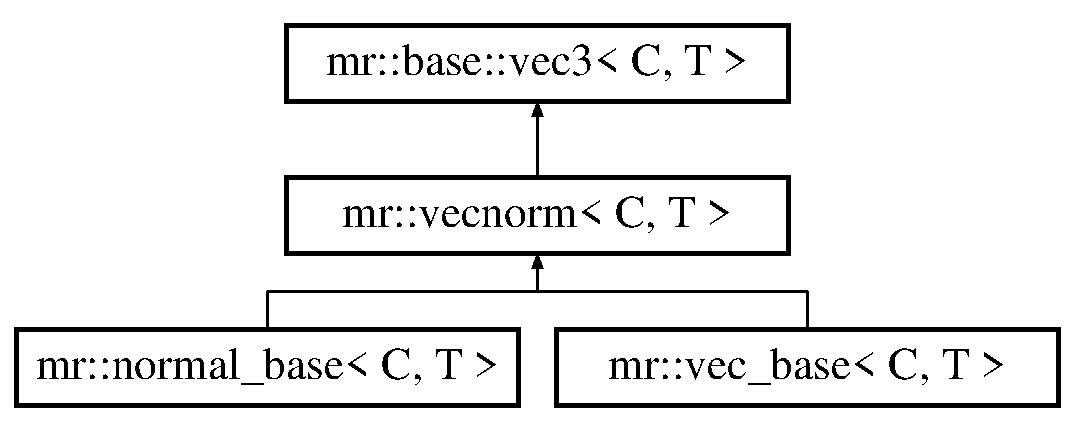
\includegraphics[height=3cm]{structmr_1_1vecnorm}
\end{center}
\end{figure}
\subsection*{Length comparisons}
\begin{CompactItemize}
\item 
bool {\bf operator$<$} (const T a) const 
\item 
bool {\bf operator$>$} (const T a) const 
\item 
bool {\bf operator$<$=} (const T a) const 
\item 
bool {\bf operator$>$=} (const T a) const 
\item 
bool {\bf operator$<$} (const {\bf vecnorm} \&a) const 
\item 
bool {\bf operator$>$} (const {\bf vecnorm} \&a) const 
\item 
bool {\bf operator$<$=} (const {\bf vecnorm} \&a) const 
\item 
bool {\bf operator$>$=} (const {\bf vecnorm} \&a) const 
\end{CompactItemize}
\subsection*{Public Types}
\begin{CompactItemize}
\item 
typedef {\bf vecnorm}$<$ C, T $>$ {\bf self}
\end{CompactItemize}
\subsection*{Public Member Functions}
\begin{CompactItemize}
\item 
{\bf vecnorm} ()
\item 
{\bf vecnorm} (const T xx, const T yy, const T zz)
\item 
T {\bf length\-Squared} () const 
\item 
T {\bf length} () const 
\item 
T {\bf inverse\-Length} () const 
\item 
T {\bf inverse\-Length\-Fast} () const 
\end{CompactItemize}
\begin{Indent}{\bf Dot product}\par
\begin{CompactItemize}
\item 
template$<$class X, class Y, class Oper$>$ T {\bf operator\%} (const {\bf base::exp}$<$ X, Y, Oper $>$ \&e) const 
\item 
T {\bf operator\%} (const mi\-Vector \&b) const 
\item 
template$<$typename X$>$ T {\bf dot} (const X \&b)
\end{CompactItemize}
\end{Indent}
\begin{Indent}{\bf Inplace operations}\par
\begin{CompactItemize}
\item 
void {\bf invert} ()
\item 
void {\bf normalize} ()
\item 
void {\bf normalize\-Fast} ()
\item 
bool {\bf is\-Normalized} () const 
\begin{CompactList}\small\item\em Return whether vector is normalized or not. \item\end{CompactList}\end{CompactItemize}
\end{Indent}
\subsubsection*{template$<$class C, typename T$>$ struct mr::vecnorm$<$ C, T $>$}



\subsection{Member Typedef Documentation}
\index{mr::vecnorm@{mr::vecnorm}!self@{self}}
\index{self@{self}!mr::vecnorm@{mr::vecnorm}}
\subsubsection{\setlength{\rightskip}{0pt plus 5cm}template$<$class C, typename T$>$ typedef {\bf vecnorm}$<$ C, T $>$ {\bf mr::vecnorm}$<$ C, T $>$::{\bf self}}\label{structmr_1_1vecnorm_w0}




Reimplemented from {\bf mr::base::vec3$<$ C, T $>$} {\rm (p.\,\pageref{structmr_1_1base_1_1vec3_w0})}.

Reimplemented in {\bf mr::vec\_\-base$<$ C, T $>$} {\rm (p.\,\pageref{structmr_1_1vec__base_w0})}, and {\bf mr::normal\_\-base$<$ C, T $>$} {\rm (p.\,\pageref{structmr_1_1normal__base_w0})}.

\subsection{Constructor \& Destructor Documentation}
\index{mr::vecnorm@{mr::vecnorm}!vecnorm@{vecnorm}}
\index{vecnorm@{vecnorm}!mr::vecnorm@{mr::vecnorm}}
\subsubsection{\setlength{\rightskip}{0pt plus 5cm}template$<$class C, typename T$>$ {\bf mr::vecnorm}$<$ C, T $>$::{\bf vecnorm} ()\hspace{0.3cm}{\tt  [inline]}}\label{structmr_1_1vecnorm_a0}


\index{mr::vecnorm@{mr::vecnorm}!vecnorm@{vecnorm}}
\index{vecnorm@{vecnorm}!mr::vecnorm@{mr::vecnorm}}
\subsubsection{\setlength{\rightskip}{0pt plus 5cm}template$<$class C, typename T$>$ {\bf mr::vecnorm}$<$ C, T $>$::{\bf vecnorm} (const T {\em xx}, const T {\em yy}, const T {\em zz})\hspace{0.3cm}{\tt  [inline]}}\label{structmr_1_1vecnorm_a1}




\subsection{Member Function Documentation}
\index{mr::vecnorm@{mr::vecnorm}!dot@{dot}}
\index{dot@{dot}!mr::vecnorm@{mr::vecnorm}}
\subsubsection{\setlength{\rightskip}{0pt plus 5cm}template$<$class C, typename T$>$ template$<$typename X$>$ T {\bf mr::vecnorm}$<$ C, T $>$::dot (const X \& {\em b})\hspace{0.3cm}{\tt  [inline]}}\label{structmr_1_1vecnorm_z55_2}


\index{mr::vecnorm@{mr::vecnorm}!inverseLength@{inverseLength}}
\index{inverseLength@{inverseLength}!mr::vecnorm@{mr::vecnorm}}
\subsubsection{\setlength{\rightskip}{0pt plus 5cm}template$<$class C, typename T$>$ T {\bf mr::vecnorm}$<$ C, T $>$::inverse\-Length () const\hspace{0.3cm}{\tt  [inline]}}\label{structmr_1_1vecnorm_a4}


\index{mr::vecnorm@{mr::vecnorm}!inverseLengthFast@{inverseLengthFast}}
\index{inverseLengthFast@{inverseLengthFast}!mr::vecnorm@{mr::vecnorm}}
\subsubsection{\setlength{\rightskip}{0pt plus 5cm}template$<$class C, typename T$>$ T {\bf mr::vecnorm}$<$ C, T $>$::inverse\-Length\-Fast () const\hspace{0.3cm}{\tt  [inline]}}\label{structmr_1_1vecnorm_a5}


\index{mr::vecnorm@{mr::vecnorm}!invert@{invert}}
\index{invert@{invert}!mr::vecnorm@{mr::vecnorm}}
\subsubsection{\setlength{\rightskip}{0pt plus 5cm}template$<$class C, typename T$>$ void {\bf mr::vecnorm}$<$ C, T $>$::invert ()\hspace{0.3cm}{\tt  [inline]}}\label{structmr_1_1vecnorm_z56_0}


\index{mr::vecnorm@{mr::vecnorm}!isNormalized@{isNormalized}}
\index{isNormalized@{isNormalized}!mr::vecnorm@{mr::vecnorm}}
\subsubsection{\setlength{\rightskip}{0pt plus 5cm}template$<$class C, typename T$>$ bool {\bf mr::vecnorm}$<$ C, T $>$::is\-Normalized () const}\label{structmr_1_1vecnorm_z56_3}


Return whether vector is normalized or not. 

\index{mr::vecnorm@{mr::vecnorm}!length@{length}}
\index{length@{length}!mr::vecnorm@{mr::vecnorm}}
\subsubsection{\setlength{\rightskip}{0pt plus 5cm}template$<$class C, typename T$>$ T {\bf mr::vecnorm}$<$ C, T $>$::length () const\hspace{0.3cm}{\tt  [inline]}}\label{structmr_1_1vecnorm_a3}


\index{mr::vecnorm@{mr::vecnorm}!lengthSquared@{lengthSquared}}
\index{lengthSquared@{lengthSquared}!mr::vecnorm@{mr::vecnorm}}
\subsubsection{\setlength{\rightskip}{0pt plus 5cm}template$<$class C, typename T$>$ T {\bf mr::vecnorm}$<$ C, T $>$::length\-Squared () const\hspace{0.3cm}{\tt  [inline]}}\label{structmr_1_1vecnorm_a2}


\index{mr::vecnorm@{mr::vecnorm}!normalize@{normalize}}
\index{normalize@{normalize}!mr::vecnorm@{mr::vecnorm}}
\subsubsection{\setlength{\rightskip}{0pt plus 5cm}template$<$class C, typename T$>$ void {\bf mr::vecnorm}$<$ C, T $>$::normalize ()\hspace{0.3cm}{\tt  [inline]}}\label{structmr_1_1vecnorm_z56_1}


\index{mr::vecnorm@{mr::vecnorm}!normalizeFast@{normalizeFast}}
\index{normalizeFast@{normalizeFast}!mr::vecnorm@{mr::vecnorm}}
\subsubsection{\setlength{\rightskip}{0pt plus 5cm}template$<$class C, typename T$>$ void {\bf mr::vecnorm}$<$ C, T $>$::normalize\-Fast ()\hspace{0.3cm}{\tt  [inline]}}\label{structmr_1_1vecnorm_z56_2}


\index{mr::vecnorm@{mr::vecnorm}!operator\%@{operator\%}}
\index{operator\%@{operator\%}!mr::vecnorm@{mr::vecnorm}}
\subsubsection{\setlength{\rightskip}{0pt plus 5cm}template$<$class C, typename T$>$ T {\bf mr::vecnorm}$<$ C, T $>$::operator\% (const mi\-Vector \& {\em b}) const\hspace{0.3cm}{\tt  [inline]}}\label{structmr_1_1vecnorm_z55_1}


\index{mr::vecnorm@{mr::vecnorm}!operator\%@{operator\%}}
\index{operator\%@{operator\%}!mr::vecnorm@{mr::vecnorm}}
\subsubsection{\setlength{\rightskip}{0pt plus 5cm}template$<$class C, typename T$>$ template$<$class X, class Y, class Oper$>$ T {\bf mr::vecnorm}$<$ C, T $>$::operator\% (const {\bf base::exp}$<$ X, Y, Oper $>$ \& {\em e}) const\hspace{0.3cm}{\tt  [inline]}}\label{structmr_1_1vecnorm_z55_0}


\index{mr::vecnorm@{mr::vecnorm}!operator<@{operator$<$}}
\index{operator<@{operator$<$}!mr::vecnorm@{mr::vecnorm}}
\subsubsection{\setlength{\rightskip}{0pt plus 5cm}template$<$class C, typename T$>$ bool {\bf mr::vecnorm}$<$ C, T $>$::operator$<$ (const {\bf vecnorm}$<$ C, T $>$ \& {\em a}) const\hspace{0.3cm}{\tt  [inline]}}\label{structmr_1_1vecnorm_z57_4}


\index{mr::vecnorm@{mr::vecnorm}!operator<@{operator$<$}}
\index{operator<@{operator$<$}!mr::vecnorm@{mr::vecnorm}}
\subsubsection{\setlength{\rightskip}{0pt plus 5cm}template$<$class C, typename T$>$ bool {\bf mr::vecnorm}$<$ C, T $>$::operator$<$ (const T {\em a}) const\hspace{0.3cm}{\tt  [inline]}}\label{structmr_1_1vecnorm_z57_0}


\index{mr::vecnorm@{mr::vecnorm}!operator<=@{operator$<$=}}
\index{operator<=@{operator$<$=}!mr::vecnorm@{mr::vecnorm}}
\subsubsection{\setlength{\rightskip}{0pt plus 5cm}template$<$class C, typename T$>$ bool {\bf mr::vecnorm}$<$ C, T $>$::operator$<$= (const {\bf vecnorm}$<$ C, T $>$ \& {\em a}) const\hspace{0.3cm}{\tt  [inline]}}\label{structmr_1_1vecnorm_z57_6}


\index{mr::vecnorm@{mr::vecnorm}!operator<=@{operator$<$=}}
\index{operator<=@{operator$<$=}!mr::vecnorm@{mr::vecnorm}}
\subsubsection{\setlength{\rightskip}{0pt plus 5cm}template$<$class C, typename T$>$ bool {\bf mr::vecnorm}$<$ C, T $>$::operator$<$= (const T {\em a}) const\hspace{0.3cm}{\tt  [inline]}}\label{structmr_1_1vecnorm_z57_2}


\index{mr::vecnorm@{mr::vecnorm}!operator>@{operator$>$}}
\index{operator>@{operator$>$}!mr::vecnorm@{mr::vecnorm}}
\subsubsection{\setlength{\rightskip}{0pt plus 5cm}template$<$class C, typename T$>$ bool {\bf mr::vecnorm}$<$ C, T $>$::operator$>$ (const {\bf vecnorm}$<$ C, T $>$ \& {\em a}) const\hspace{0.3cm}{\tt  [inline]}}\label{structmr_1_1vecnorm_z57_5}


\index{mr::vecnorm@{mr::vecnorm}!operator>@{operator$>$}}
\index{operator>@{operator$>$}!mr::vecnorm@{mr::vecnorm}}
\subsubsection{\setlength{\rightskip}{0pt plus 5cm}template$<$class C, typename T$>$ bool {\bf mr::vecnorm}$<$ C, T $>$::operator$>$ (const T {\em a}) const\hspace{0.3cm}{\tt  [inline]}}\label{structmr_1_1vecnorm_z57_1}


\index{mr::vecnorm@{mr::vecnorm}!operator>=@{operator$>$=}}
\index{operator>=@{operator$>$=}!mr::vecnorm@{mr::vecnorm}}
\subsubsection{\setlength{\rightskip}{0pt plus 5cm}template$<$class C, typename T$>$ bool {\bf mr::vecnorm}$<$ C, T $>$::operator$>$= (const {\bf vecnorm}$<$ C, T $>$ \& {\em a}) const\hspace{0.3cm}{\tt  [inline]}}\label{structmr_1_1vecnorm_z57_7}


\index{mr::vecnorm@{mr::vecnorm}!operator>=@{operator$>$=}}
\index{operator>=@{operator$>$=}!mr::vecnorm@{mr::vecnorm}}
\subsubsection{\setlength{\rightskip}{0pt plus 5cm}template$<$class C, typename T$>$ bool {\bf mr::vecnorm}$<$ C, T $>$::operator$>$= (const T {\em a}) const\hspace{0.3cm}{\tt  [inline]}}\label{structmr_1_1vecnorm_z57_3}




The documentation for this struct was generated from the following file:\begin{CompactItemize}
\item 
{\bf mr\-Vector.h}\end{CompactItemize}
